Neste capítulo é disponibilizada toda a implementação do trabalho assim 
como as configurações do ambiente computacional em que foi desenvolvida. 
Também são explicitados bibliotecas e demais \textit{softwares} 
utilizados que, juntamente com o \textit{software} desenvolvido, compõem o 
sistema investigado.

\section{\textit{Software}}

Todo o software desenvolvido neste trabalho, utilizado nas investigações 
e na experimentação, está disponibilizado no 
repositório \url{https://github.com/wvmcastro/slam} sob licença de uso 
GPLv3 que permite a todos utilizá-lo e modificá-lo livremente.

Toda a teoria apresentada nos capítulos \ref{ch:back-end}, \ref{ch:front-end} e \ref{ch:distributed-slam} foi implementada; a única 
exceção é a exploração autônoma apresentada na Seção \ref{sec:autonomous-exploration}, na qual foram usados utilitários da 
biblioteca de navegação \cite{marder2010office} presente no Sistema 
Operacional de Robôs (ROS).

Grande parte da implementação foi feita na linguagem C++ por conta de 
seu alto desempenho e também pela série de verificações estáticas 
realizadas por seu compilador, o que evita uma enorme quantidade de 
erros de execução. Para garantir o consumo reduzido de memória viabilizado 
pelo SEIF através do emprego de matrizes esparsas, foi utilizada versão 3.3.7 
da biblioteca de álgebra linear Eigen \cite{eigen-lib} disponível para a linguagem de programação C++. As implementações 
de visualizações de gráficos foram realizadas na linguagem Python versão 
3, utilizando a biblioteca Matplotlib \cite{hunter2007matplotlib}.

\section{Ambiente computacional}

As Seções \ref{sec:env-hardware} e \ref{sec:env-software} descrevem em 
detalhes o \textit{hardware} e \textit{software} utilizados durante o 
desenvolvimento da pesquisa com o objetivo de guiar e/ou servir de 
ponto de partida para futuras pesquisas em temas relacionados a este 
trabalho.

\subsection{\textit{Hardware}}
\label{sec:env-hardware}
Tanto para o desenvolvimento quanto para a execução de experimentos foi 
utilizado um \textit{laptop} da marca Dell modelo G7 com as seguintes 
configurações:
\begin{itemize}
  \item Processador: Intel® Core\textsuperscript{TM} i7-8750H CPU @ 2.20GHz $\times$ 12
  \item Placa de vídeo: nVidia GP106M (GeForce GTX 1060 \textit{Mobile})
  \item Memória RAM: \begin{itemize}
    \item Capacidade: 16 gigabytes
    \item Modelo: DDR4
    \item Velocidade: 2400 MT/s
  \end{itemize}
  \item Memória não volátil: \begin{itemize}
    \item Disco rígido (\textit{hard drive}): TOSHIBA MQ02ABF1, capacidade de 1 terabyte
    \item Unidade de estado sólido (SSD): Micron 1100 SATA M.2, capacidade de 256 gigabytes
  \end{itemize}
\end{itemize}

\subsection{\textit{Software}}
\label{sec:env-software}
O \textit{hardware} descrito na Seção \ref{sec:env-hardware} foi equipado 
com os seguintes \textit{softwares}:
\begin{itemize}
  \item Sistema Operacional: Linux, distribuição Ubuntu 20.04 LTS
  \item \textit{Robot Operating System (ROS)} 1, versão \textit{Noetic Ninjemys}
  \item Simulador Gazebo clássico versão 11
\end{itemize}

\section{Simulação}
\subsection{O ambiente}
O ambiente consiste em uma espaço de 100$m^2$ delimitado por paredes e diversos ``postes'' de formato cilíndrico de 16$cm$ de diâmetro, e está representado na Figura \ref{fig:environment}.
\begin{figure}[h]
  \begin{subfigure}{.50\textwidth}
    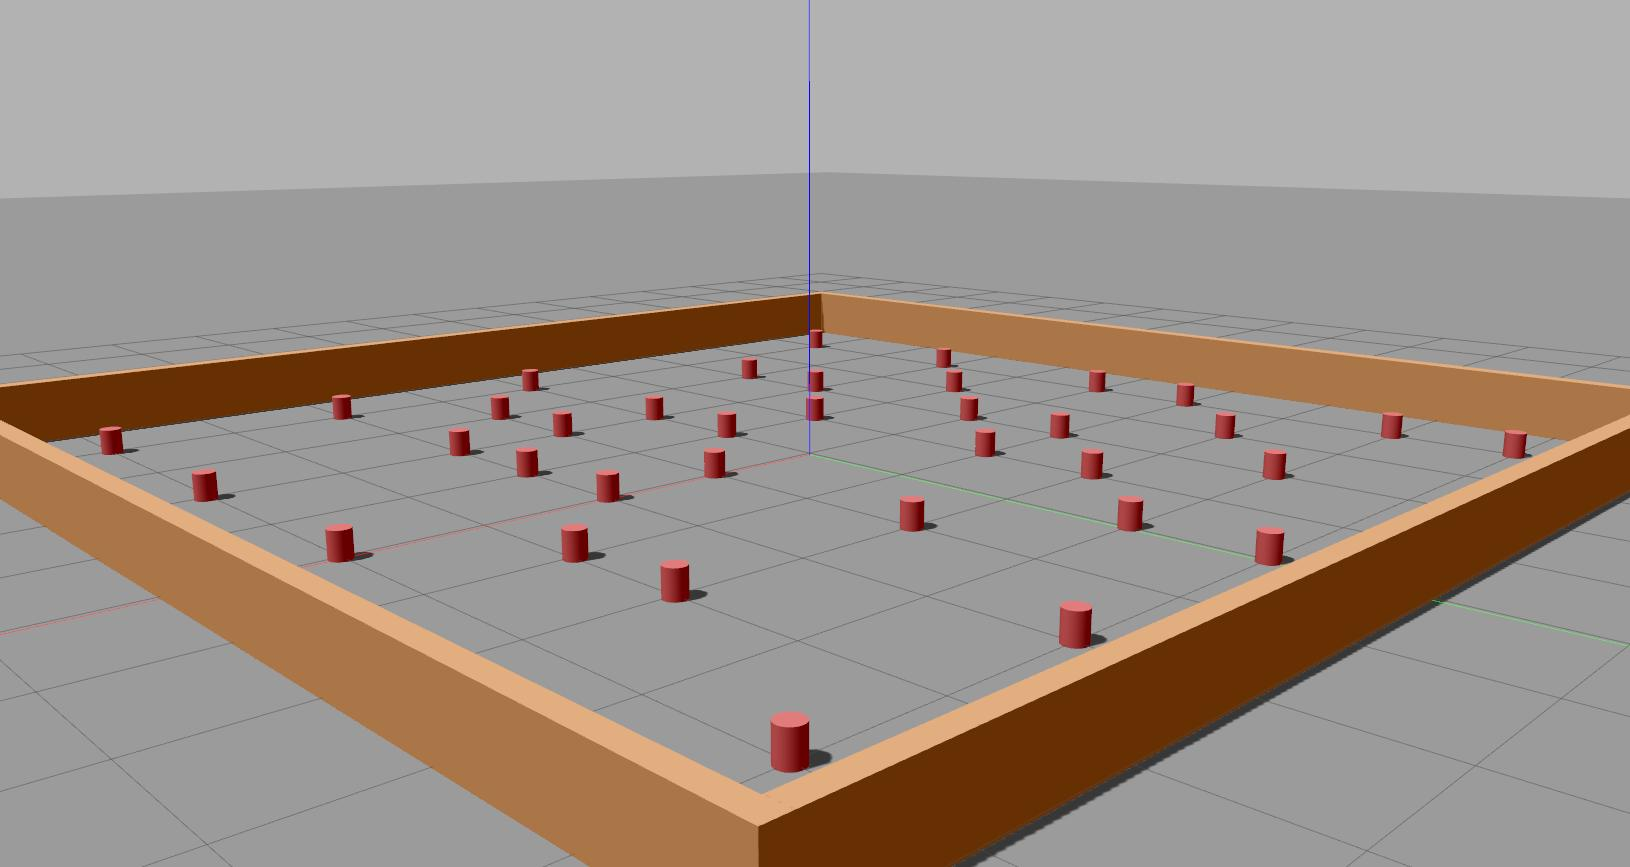
\includegraphics[width=\textwidth]{figs/environment-perspective.jpg}
    \caption{Vista perspectiva ampla}
  \end{subfigure}
  \hfill
  \begin{subfigure}{.50\textwidth}
    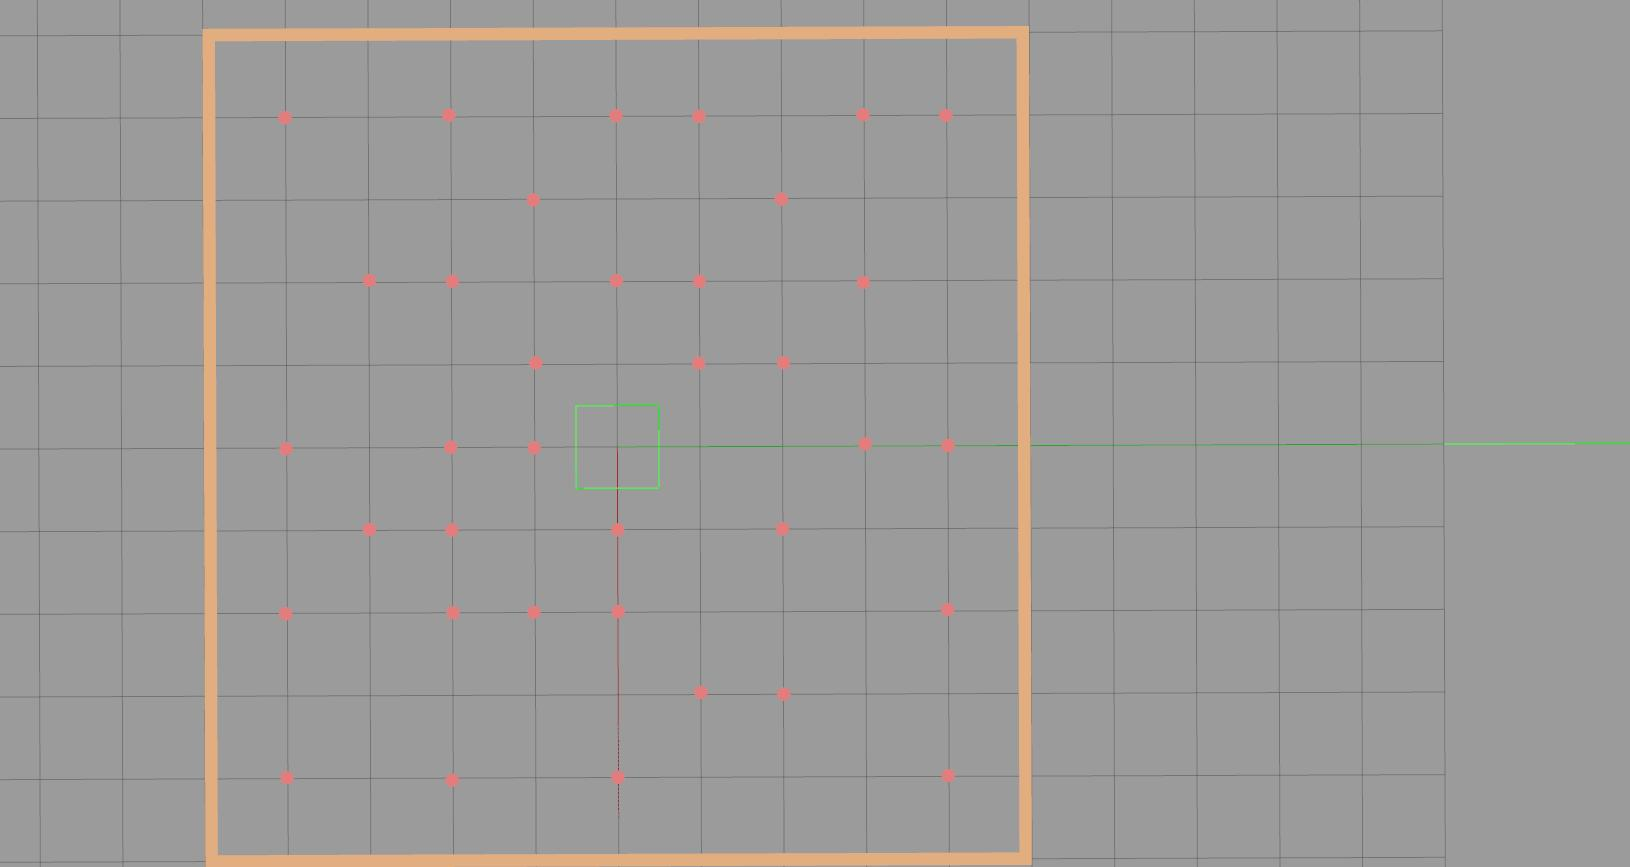
\includegraphics[width=\textwidth]{figs/environment-birds-eye-of-view.jpg}
    \caption{Vista ortográfica superior}
  \end{subfigure}
  \hfill
  \begin{subfigure}{\textwidth}
    \centering
    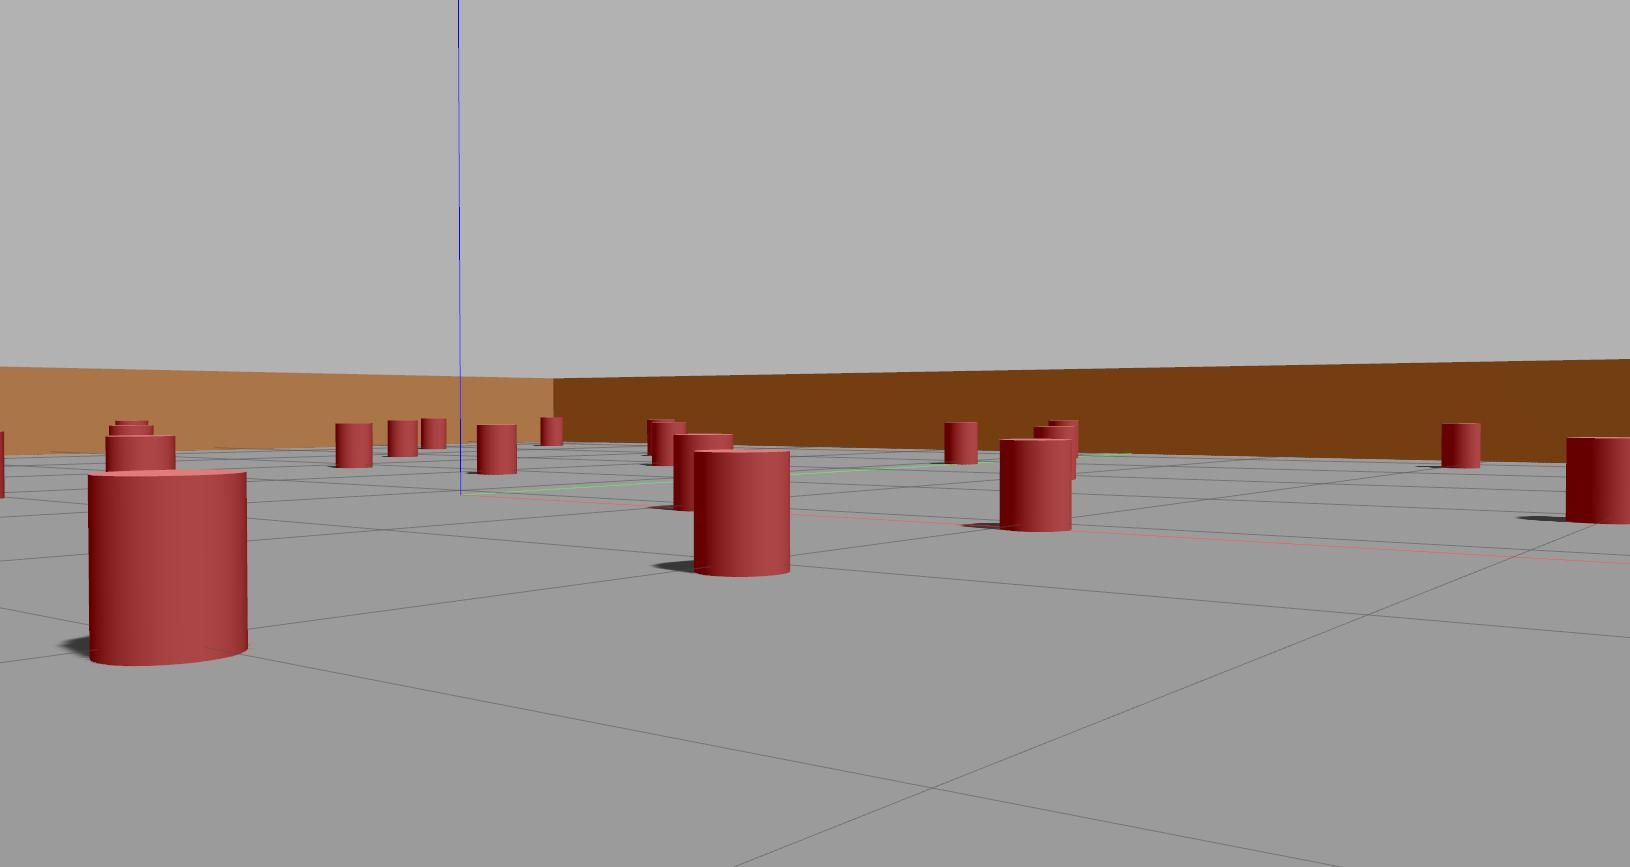
\includegraphics[width=.5\textwidth]{figs/environment-closer-perspective.jpg}
    \caption{Vista perspectiva fechada}
  \end{subfigure}
  \caption{Diferentes vistas do ambiente simulado}
  \label{fig:environment}
\end{figure}

\subsection{O robô}
Neste trabalho foi utilizado o modelo do robô \emph{Turtlebot 3} \cite{TurtleBot_3} exibido na Figura \ref{fig:turtlebot-digital-twin}, que é um robô de acionamento diferencial equipado com 
\textit{encoder} de rodas, uma IMU e um sensor laser do tipo LiDAR.
\begin{figure}[h]
  \centering
  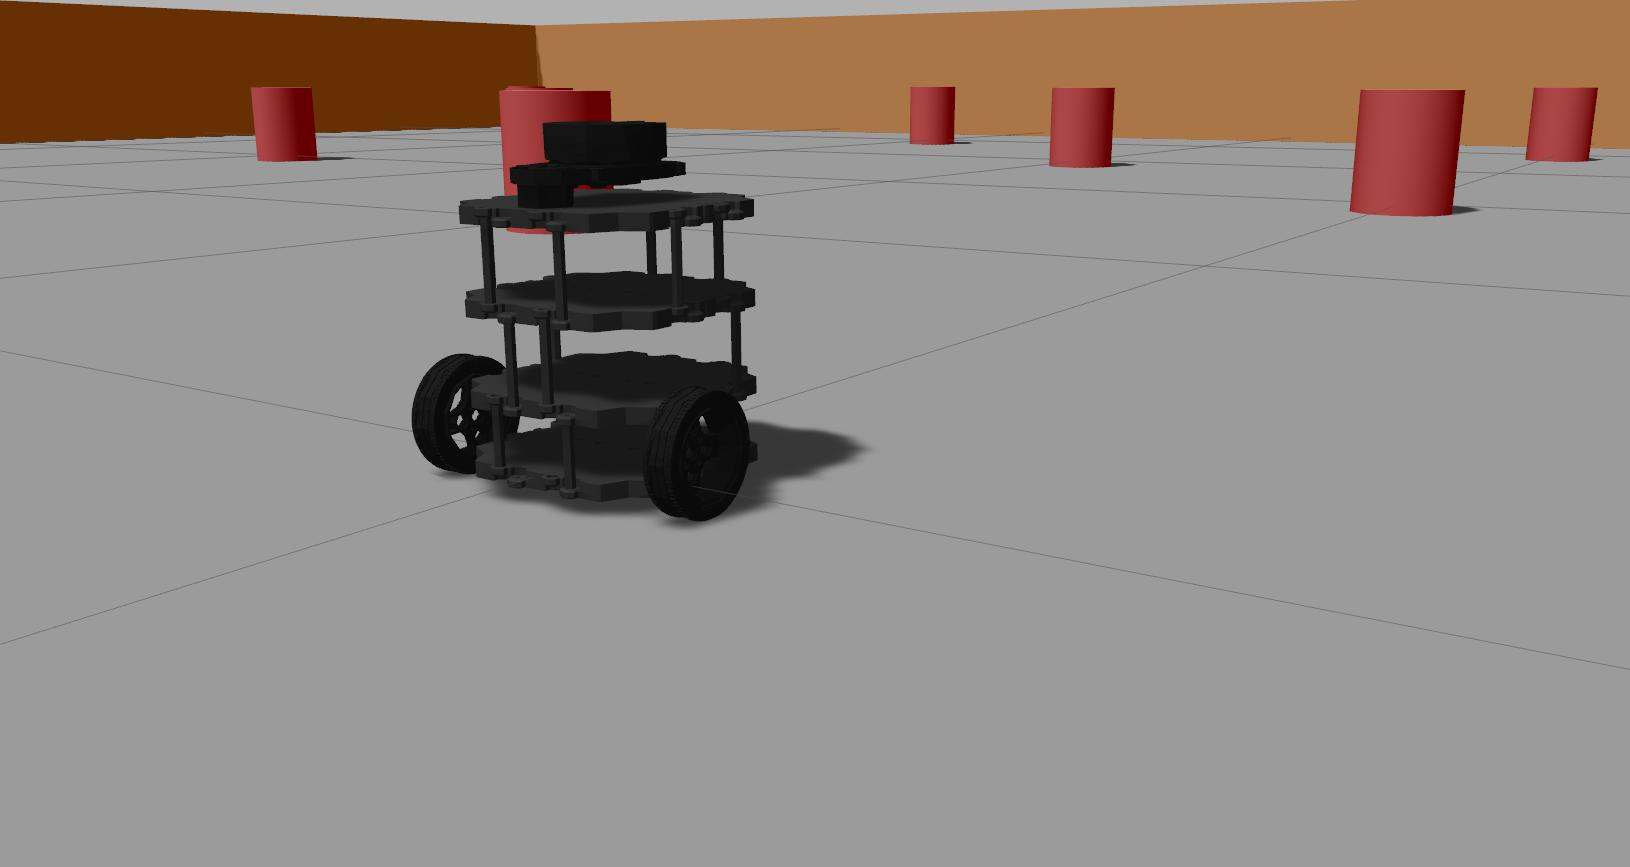
\includegraphics[width=0.7\textwidth]{figs/robot-closeup.jpg}
  \caption[Modelo do robô \textit{Turtlebot 3}]{Modelo do robô \textit{Turtlebot 3}. O sensor LiDAR encontra-se no topo do robô.}
  \label{fig:turtlebot-digital-twin}
\end{figure}

